\documentclass[10pt,twocolumn,letterpaper]{article}

\usepackage{cvpr}
\usepackage{times}
\usepackage{epsfig}
\usepackage{graphicx}
\usepackage{amsmath}
\usepackage{amssymb}
\usepackage{hyperref}

% Include other packages here, before hyperref.

% If you comment hyperref and then uncomment it, you should delete
% egpaper.aux before re-running latex.  (Or just hit 'q' on the first latex
% run, let it finish, and you should be clear).
\usepackage[pagebackref=true,breaklinks=true,letterpaper=true,colorlinks,bookmarks=false]{hyperref}

\cvprfinalcopy % *** Uncomment this line for the final submission

\def\cvprPaperID{****} % *** Enter the CVPR Paper ID here
\def\httilde{\mbox{\tt\raisebox{-.5ex}{\symbol{126}}}}

% Pages are numbered in submission mode, and unnumbered in camera-ready
\ifcvprfinal\pagestyle{empty}\fi
\begin{document}

%%%%%%%%% TITLE
\title{Project Report : CS 7643\\Differential Privacy}

\author{Krishna Kumar\\
Georgia Institute of Technology\\
Atlanta, Georgia\\
{\tt\small kkumar80@gatech.edu}
% For a paper whose authors are all at the same institution,
% omit the following lines up until the closing ``}''.
% Additional authors and addresses can be added with ``\and'',
% just like the second author.
% To save space, use either the email address or home page, not both
\and
Sumit Machwe\\
Georgia Institute of Technology\\
Atlanta, Georgia\\
{\tt\small smachwe3@gatech.edu}
}

\maketitle
%\thispagestyle{empty}

%%%%%%%%% ABSTRACT
\begin{abstract}

   % PROBLEM STATEMENT, PROPOSED SOLUTION and RESULTS

   Differential Privacy ensures to protect the private data such as social security
   numbers, age, gender, or any sensitive information (PII - Personally Identifiable Information) which can identify the individual
   persons in the dataset. This has wide applicability in domains such as
   finance, healthcare, demographic data, etc. \cite{2} \\
   Our project demonstrates the use of Differential Privacy on a Bank Credit Card Fraud detection dataset provided on Kaggle\cite{1}. This will improve the fraud detection identification by encouraging banks, financial institutions to share the data in an differential private way, so that federated learning can be done for fraud detection and solve the class imbalance (less percentage of fraud for individual bank).
   % Differential Privacy is one of the latest emerging breakthrough technologies in
   % 2020 [3]. Differential Privacy strives to create a synthetic dataset with
   % distributional similarity to the real dataset and a machine learning utility
   % sub-optimal to the real dataset (within a defined threshold).\\
   % PROPOSED SOLUTION
   Given above dataset, our project will generate a synthetic dataset that will have distributional similarity as real dataset, and Machine Learning utility which could be sub optimal to the real dataset performance by some threshold. We will demostrate distributional similarity using KDE Plots and feature correlation plots. ML utility will be demonstrated by comparing performance of real vs. synthetic dataset using AUC and F1 score.\\
   % RESULTS

\end{abstract}

%%%%%%%%% BODY TEXT
\section{Introduction/Background/Motivation}

Across industry there is always a need for sharing the data which can help in solving complex problems, such as medical drug discovery, financial fraud prevention, network security while providing end user services etc. All these cases contain PII information such as age, gender, location, ipaddress etc that discourages sharing of data and collaboration.  \\
The problem we tried to solve was to generate a synthetic dataset from a given fraud detection dataset of a bank. This synthetic dataset will have similar data distribution and machine learning utility as real dataset without compromising PII.

Data Anonymization (3-way or 5-way) is the standard practice today to protect PII. Today's data disclosure practices aim to address this issue by minimizing the number of attributes that are particularly vulnerable to re-identification. However it is prone to reverse attack where alternative datasources could be linked with anonymized data to identify the person. For example:
\begin{itemize}
    \item 87\% of Americans (based on 2010 US Census data) can be uniquely identified with only three pieces of data: Gender, Birthday and Zip Code. This is the reason why 2020 Census data is being released in a differential private dataset.

    % TODO: Provide citation
    \item  University of Texas at Austin demonstrated reverse attack on anonimized dataset provided by Netflix in 2006. UT Austin linked the anonimized dataset to the publicly available IMDB dataset and were able to uncover many customer names.
\end{itemize}

There is wide applicability across industries to protect PIIs. Institutions and organizations will collaborate more by sharing the data for solving industrial problems while not compromising customer sensitive information. Individuals will be encouraged to participate in surveys without the concern of their information being compromised. Government agencies and regulators will be able to protect citizen data, for example, implement GDPR while sharing their data.
%TODO: add GDPR link

We will use the \textbf{Bank Account Fraud Dataset Suite (NeurIPS 2022)}\cite{1} dataset provided on Kaggle. \\

This suite of datasets is based on recommendation \href{https://arxiv.org/abs/1803.09010}{here}:
\begin{itemize}
    \item Realistic, based on a present-day real-world dataset for fraud detection.
    \item Biased, each dataset has distinct controlled types of bias. Imbalanced, this setting presents a extremely low prevalence of positive class
    \item Dynamic, with temporal data and observed distribution shifts.
    \item Privacy preserving, to protect the identity of potential applicants we have applied differential privacy techniques (noise addition), feature encoding and trained a generative model (CTGAN).
    \item This dataset meets the \href{https://arxiv.org/abs/1803.09010}{section 3.1 motivations} of creating the training data for the model, such as purpose, creator and funding of dataset.
\end{itemize}

This dataset provides multiple variants. However, for our experimentation, we will only use the following variants:
\begin{itemize}
    \item Variant-V: Has \textbf{better separability in train} for one of the groups.
\end{itemize}


\section{Approach}

\begin{itemize}
    \item \textbf{EDA}\label{sec:Approach_EDA}: Analyze and visualize the dataset. Cleanup null values, convert datatypes, identified categorical variables and visualize the data distribution. We realized that the original dataset was 1 million records with more than 40 columns. Given the compute resource limitations we decided to reduce the data size from 1 million to 300,000 records. We used the \textit{stratify} parameter of the \verb'train_test_split' of sklearn library on \verb'FRAUD_BOOL' label. We also reduced the number of columns (features) based on correlation plot, retaining any feature that has $\pm0.2$ correlation with \verb'FRAUD_BOOL'. This also helped to avoid Multicollinearity.

    \item \textbf{Baseline ML Utility}: We trained \verb'Random Forest', \verb'Naive Bayes' and \verb'Logistic Regression' models on the real (reduced) dataset. Evaluated and plotted the Precision, Recall, F1 score and AUC/ROC. This provided us the ML utility baseline performance. This should act as an upperbound on the synthetic dataset generated by our our implementation of Differential Privacy.

    \item \textbf{Main Algorithm for Differential Privacy:}
    Differential Privacy is a randomized algorithm $(K)$, which gives \\$\epsilon\text{-differential \ privacy}$ if for all data sets $D$ and $D'$ differing on at most one row, and any $S \subseteq Range(K)$ , \cite{4} $$Pr[K(D) \in S] \leq exp(\epsilon) \times \text{Pr}[K(D')] \in S'$$

        Following two quantities must be considered in DP algorithms:
        \begin{itemize}
            \item Epsilon ($\epsilon$): A metric of privacy loss at a differentially change in data (adding or removing 1 entry). The smaller the value, the better privacy protection.

            \item Accuracy: The closeness of the output of DP algorithms to the pure output measured by \text{PMSE ratio} \cite{5}

        \end{itemize}

    \item In order to identify the optimal DP model, we trained all three models (DP-CTGAN, PATE-CTGAN and QUAIL) on $\epsilon=3.0$. For QUAIL we used DP-Naive Bayes as its classifier and used DP-CTGAN and PATE-CTGAN as its synthesizers.

    \item \textbf{Algorithm Implementation}: As a first step, we created base models using default hyper-parameters and $\epsilon=3.0$. We evaluated the model performance and ML utility (Precision, Recall, ROC-AUC, F1 score) using below tests. %TODO Provide link)
    \begin{itemize}
        \item \verb'TRTR': \textit{Train Real Test Real}
        \item \verb'TSTR': \textit{Train Synthetic Test Real}
        \item \verb'TSTS': \textit{Train Synthetic Test Synthetic}
    \end{itemize}

    \item We compared base model performance on \verb'TRTR' vs. \verb'TSTR'. \\
    \verb'TSTR' performance is expected to be sub-optimal to \verb'TRTR' but not overfit. However, \verb'TSTS' performance is expected to be the best, but overfit. Hence we decided to use \verb'TSTR' performance as the baseline model performance. \\

    \item Based on the base model performance comparisons \verb'DP-CTGAN' synthesizer has better performance than \verb'PATE-CTGAN'. Our test observed that QUAIL with \verb'DP-CTGAN' and \verb'PATE-CTGAN' synthesizers was creating a single class for \verb'FRAUD-BOOL'. Hence we decided to drop QUAIL from further experimentation for this dataset.

    \item We then selected \verb'DP-CTGAN' and \verb'PATE-CTGAN' for further experimentation (change $\epsilon=10.0$ and keep other parameters intact) and repeated above steps for comparing the model performance.

    \item Model performance improved in the new $\epsilon=10.0$. We again observed performance of \verb'DP-CTGAN' to be better than that of \verb'PATE-CTGAN'.

    \item Hence we decided to do various hyper-parameter tuning on \verb'DP-CTGAN' in pursuit of finding the best model (in terms of ML Utility and Distributional Similarity). Experiments and Results section has further details on hyper-parameter tuning.

    \item Above experiments would be successful because we are trying to recursively narrow down on synthesizers with various test setup to find an optimal model which produces a synthetic dataset which is close to the real dataset only by data distribution and ML utility. This is a standard approach for differential privacy.


    \item Synthetic dataset would have a distributional similarity. We will demonstrate this by using KDE Plot and histograms. We will use the \text{PMSE ratio} as a measure.\cite{5}

    \item We will run ML models (Logistic Regression, Random Forest, Decision Tree, and Naive Bayes) and compare and contrast the performance of:
    \begin{itemize}
        \item $TRTR$: \textit{Train Real Test Real}
        \item $TSTR$: \textit{Train Synthetic Test Real}
        \item $TSTS$: \textit{Train Synthetic Test Synthetic}
    \end{itemize}

    \item Our approach requires hyperparameter tuning to find optimal parameters.
\end{itemize}

    \item \textbf{Problem Anticipation}:
    \begin{itemize}
        \item We anticipated the runtime environment creation of Differential Privacy would be challenging due to strict library version requirements. It took more than 3 days to setup the correct set of libraries, conda environment creation.
        \item We also anticipated the creation of runtime environment in Cloud (GCP) would have a learning curve specially given the library versions. Local setup worked, however we could not port the setup to GCP or Google Colab. Created an Ed Discussion post, but could not solicit any good solution. Hence we decided to work on local environment for training GANs.
        \item Training GANs require heavy resource: GPUs, Memory and computation time. We found training on GANs is extremely time consuming. Most of the experiments took 12 to 14 hours to finish. Many experiments failed due to kernel crashes and required restarts. Local setup had no ability to parallize experiments, which slowed us down. We ultimately ended up running the expeiments on on 4 M1 Macbook Pro (32 GB CPU mem/ 8GB GPU mem) laptops.
        \item We expected \verb'TSTS' test performance to overfit. Our experiments confirmed our anticipation. Hence we chose to use \verb'TSTR' as our metrics for comparison.
        \item We expected to run numerous experiments to find the best model with optimal hyper-parameters. Although we ran 10 experiments, we really could not find better model performance than the baseline model. We could have expanded our hyper-parameter search if we had more time and resources in terms of hardware (GPUs and parallelization).
    \end{itemize}


\textbf{Important: Mention any code repositories (with citations) or other sources that you used, and specifically what changes you made to them for your project. }

\section{Experiments and Results}

\begin{itemize}
    \item We applied Differential Privacy algorithms on the reduced dataset (\hyperref[sec:Approach_EDA]{Please refer to EDA in Approach section}).
    %TODO: Add correlation plot fig and hyperlink with approach section \

    \item Trained \verb'Random Forest', \verb'Naive Bayes', and \verb'Logistic Regression' models on the real (reduced) dataset and evaluated its performance using these metrics: \verb'Precision', \verb'Recall', \verb'F1 score', and \verb'AUC/ROC'). As discussed in Apporach section, this is the \verb'TRTR model' (Train Real, Test Real with 70:30 split).
    %TODO: Create Excel spreadsheet, take an image. Ensure to populate all 4 metrics and their results

    \item As Discussed in the approach section, For Synthetic data created using differential privacy,  We calculate \verb'Precision', \verb'Recall', \verb'F1 score', and \verb'AUC/ROC').
    %TODO: Combine this item with the item above. Essentially represent the results of synthetic data in the same or different table above.

    \item To measure the success of our approach, we compared ML metrics of TSTR. We also published results for \verb'TSTS' (Train Synthetic, Test Synthetic - with 70:30 split)

    \item For distributional similarity between real and synthetic datasets, we measure it through KDE plots and pMSE ratios.
    %TODO: apply the images from KDE plots and create the table for pMSE Scores.

    \item \textbf{Baseline Solution}: Train the baseline models with $\epsilon=3.0$ and $\epsilon=5.0$. Please find below ML Utility and PMSE Ratios.
    %and KDE plots. We also plotted the Loss Functions for Generator and Discriminators.

    \begin{figure}[ht]
    \begin{center}
       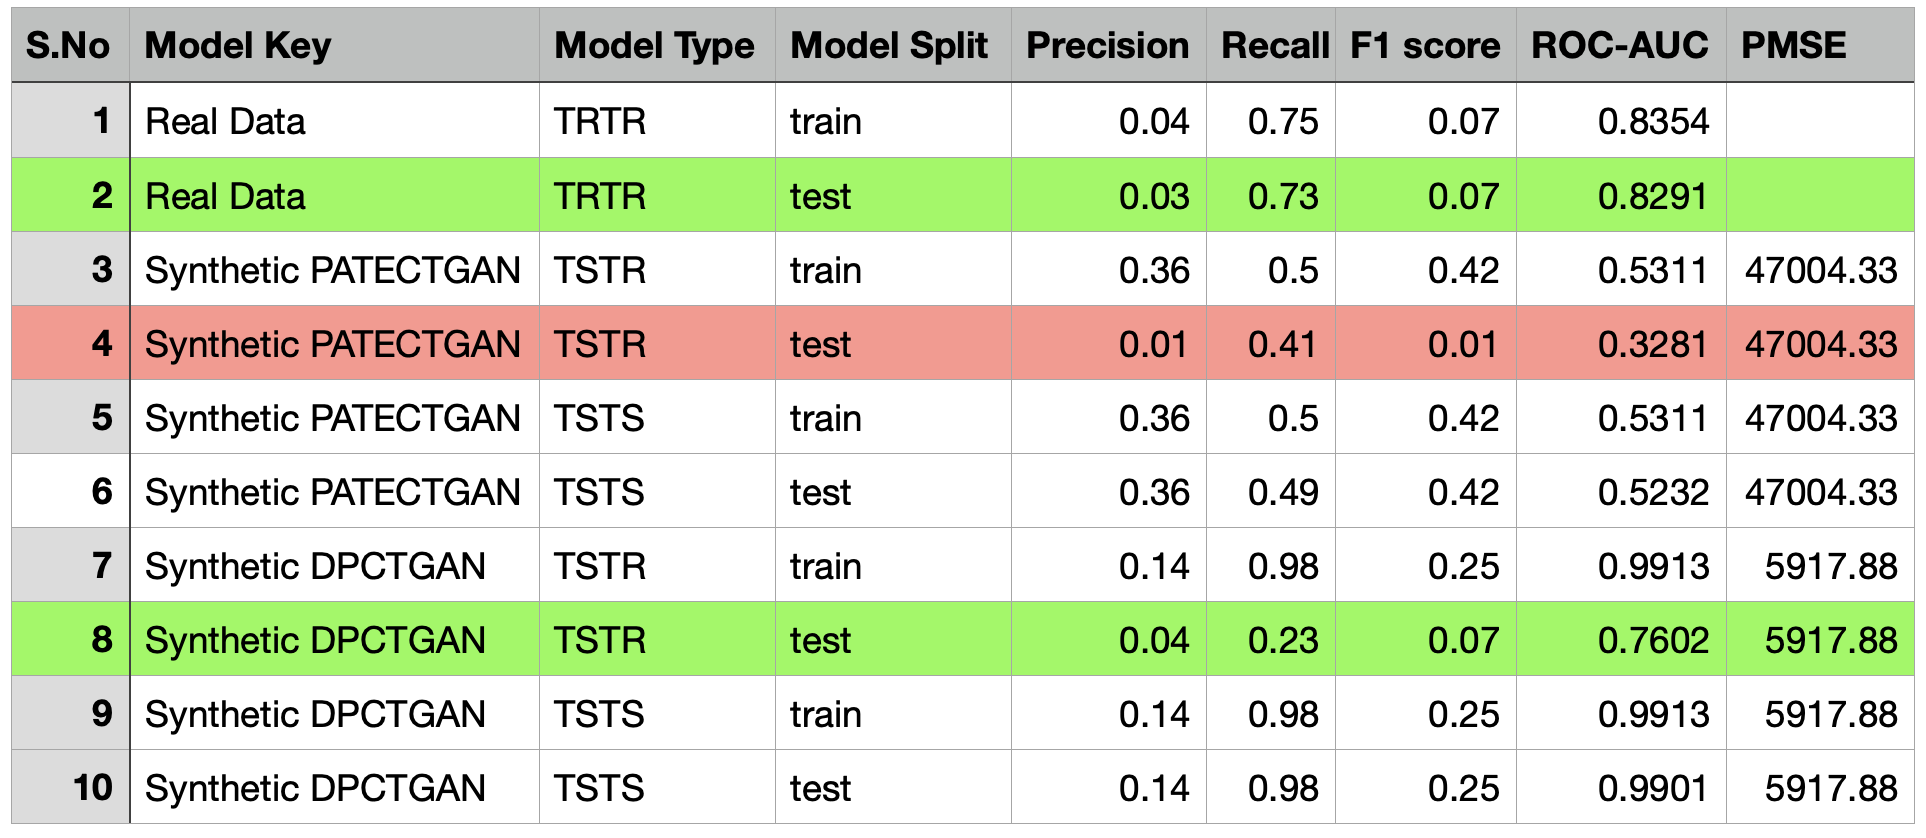
\includegraphics[width=0.8\linewidth]{Baseline_ML_Utility_Epsilon_3.0.png}
    \end{center}
       \caption{Baseline ML Utlity Performance metrics. Real Dataset with 300K rows and 11 features. Synthetic Dataset with $\epsilon=3.0$. Best model: DPCTGAN}
    \label{fig:long}
    \label{fig:onecol}
    \end{figure}

    \begin{figure}[ht]
    \begin{center}
       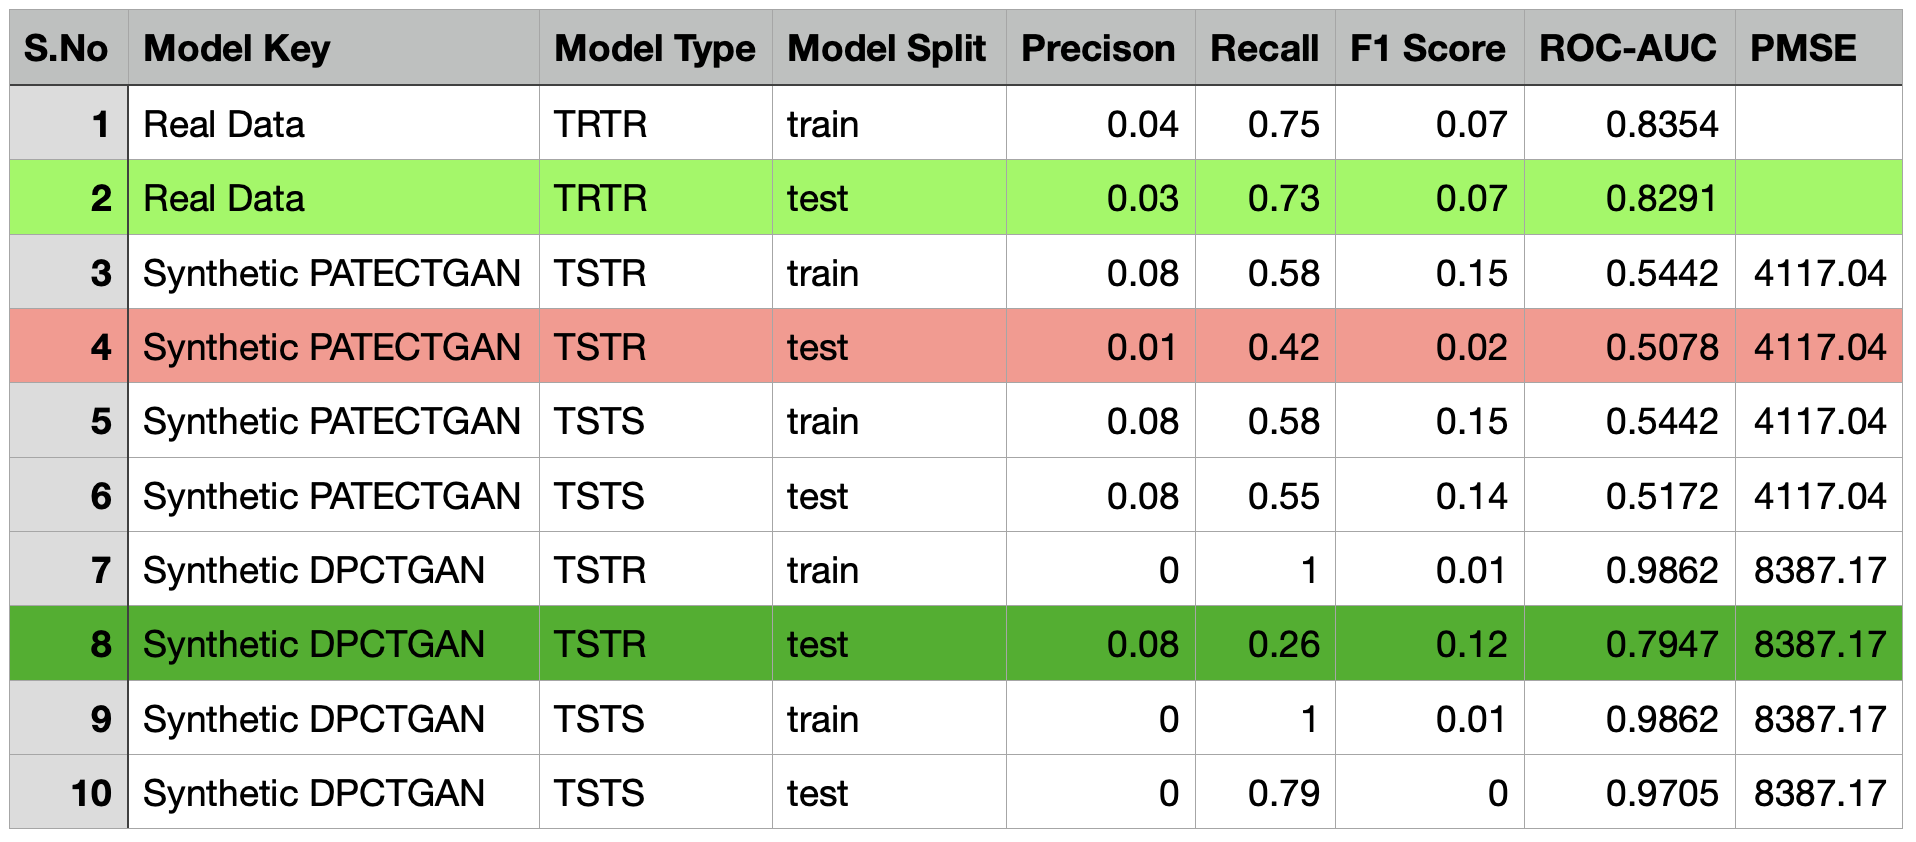
\includegraphics[width=0.8\linewidth]{Baseline_ML_Utility_Epsilon_5.0.png}
    \end{center}
       \caption{Baseline ML Utlity Performance metrics. Real Dataset with 300K rows and 11 features. Synthetic Dataset with $\epsilon=5.0$. \textbf{Champion model: DPCTGAN}}
    \label{fig:long}
    \label{fig:onecol}
    \end{figure}
\end{itemize}

\begin{itemize}

    \item \textbf{Hyperparameter Tuning} We conducted 12 experiments. Please find below ML Utility, PMSE Ratios metrics for experiments having comparable results with real dataset.
    %TODO: Show the table of 12 experiments here
    \begin{figure}[ht]
    \begin{center}
       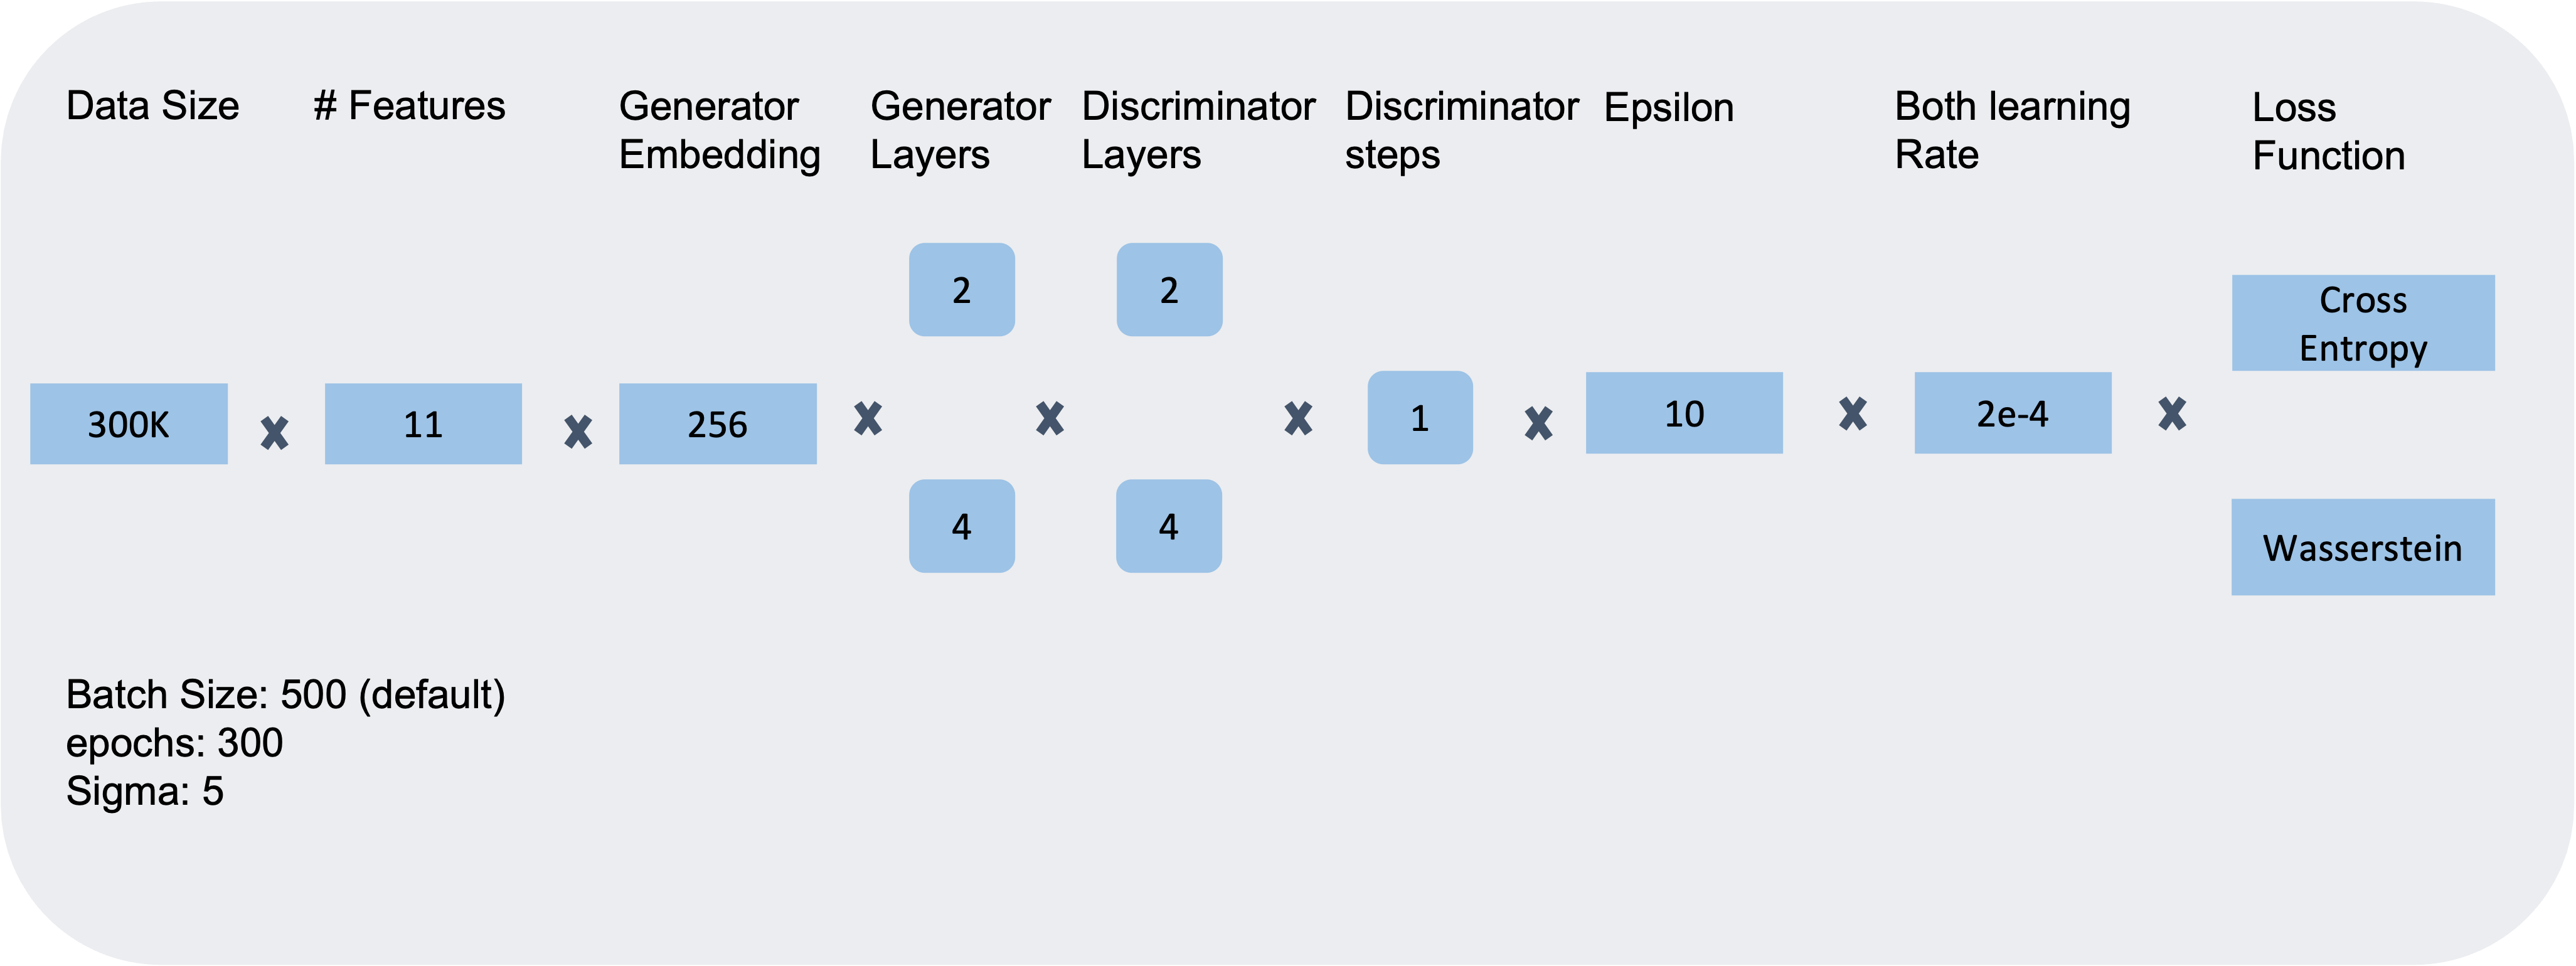
\includegraphics[width=0.9\linewidth]{DP-CTGAN.png}
    \end{center}
    %TODO: add caption
       \caption{Experiment Designs. Base experiments were conducted as above. In addition, we conducted specific experiments to achieve better performance. Details described in next figure.}.
    \label{fig:long}
    \label{fig:onecol}
    \end{figure}

    \begin{figure}[ht]
    \begin{center}
       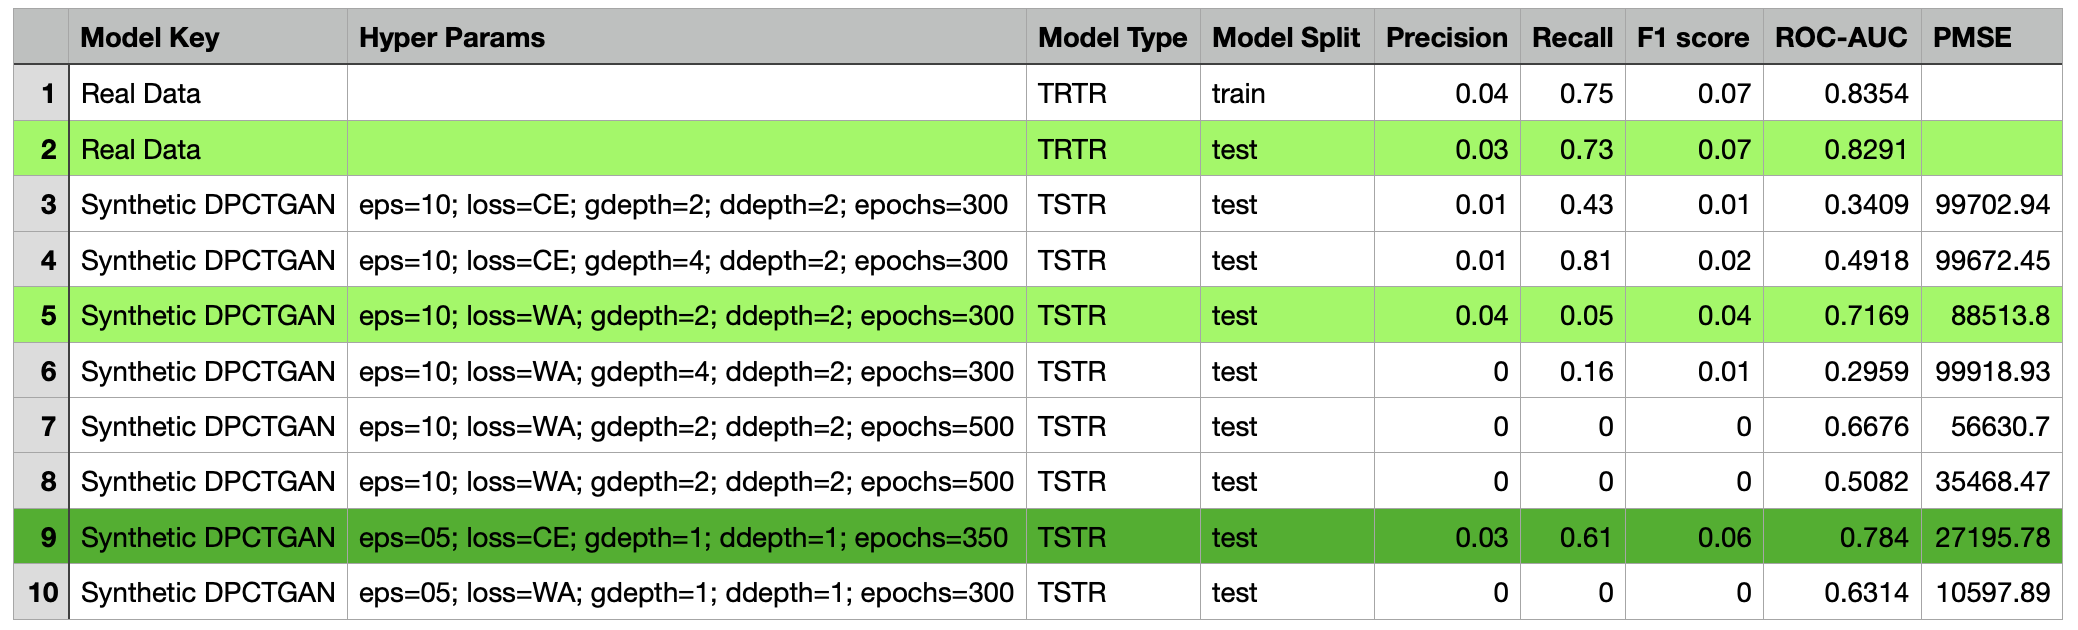
\includegraphics[width=0.9\linewidth]{Hyperparameter_ML_Utility_Epsilon_5_10.png}
    \end{center}
    %TODO: add caption
       \caption{Hyperparamter Tuning ML Utility Performance metrics.}
    \label{fig:long}
    \label{fig:onecol}
    \end{figure}

    \item Based on all above experiments, baseline model with synthesizer DPCTGAN, $epsilon=5.0$ is the champion model for the given dataset. Please find its ML Utility and KDE plots.
    \begin{figure}[ht]
        \begin{center}
           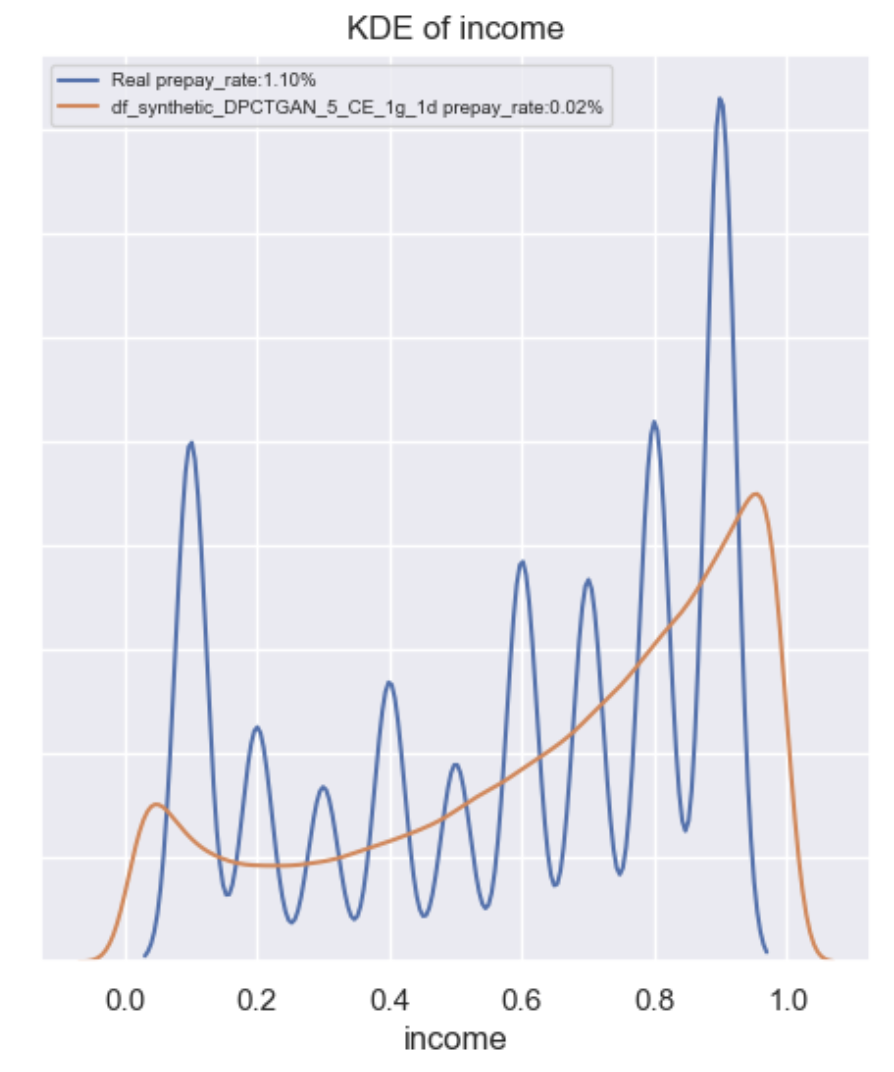
\includegraphics[width=0.5\linewidth]{Income_KDE_Plot.png}
        \end{center}
        %TODO: add caption
           \caption{Real vs. Synthetic data KDE Plot: Income}
        \label{fig:long}
        \label{fig:onecol}
    \end{figure}
    \begin{figure}[ht]
        \begin{center}
           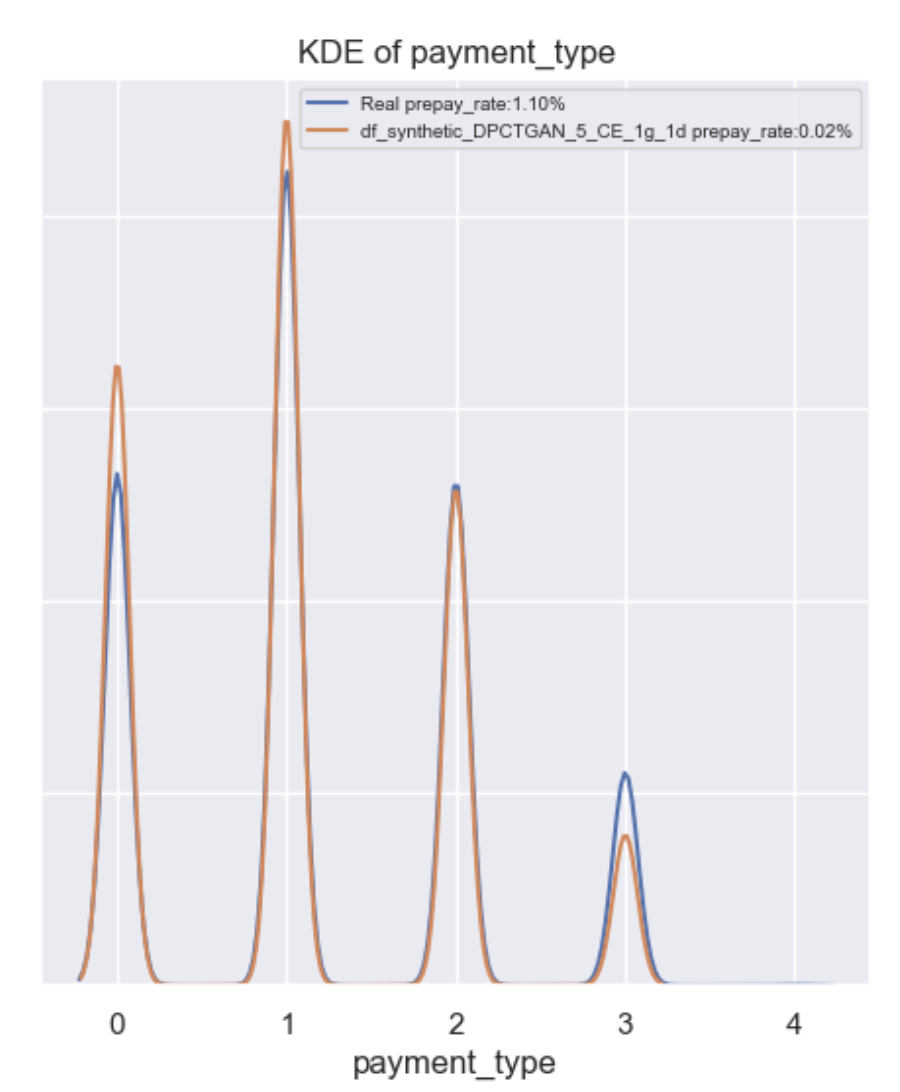
\includegraphics[width=0.5\linewidth]{Payment_Type_KDE_Plot.png}
        \end{center}
        %TODO: add caption
           \caption{Real vs. Synthetic data KDE Plot: Payment Type}
        \label{fig:long}
        \label{fig:onecol}
    \end{figure}
    \begin{figure}[ht]
        \begin{center}
           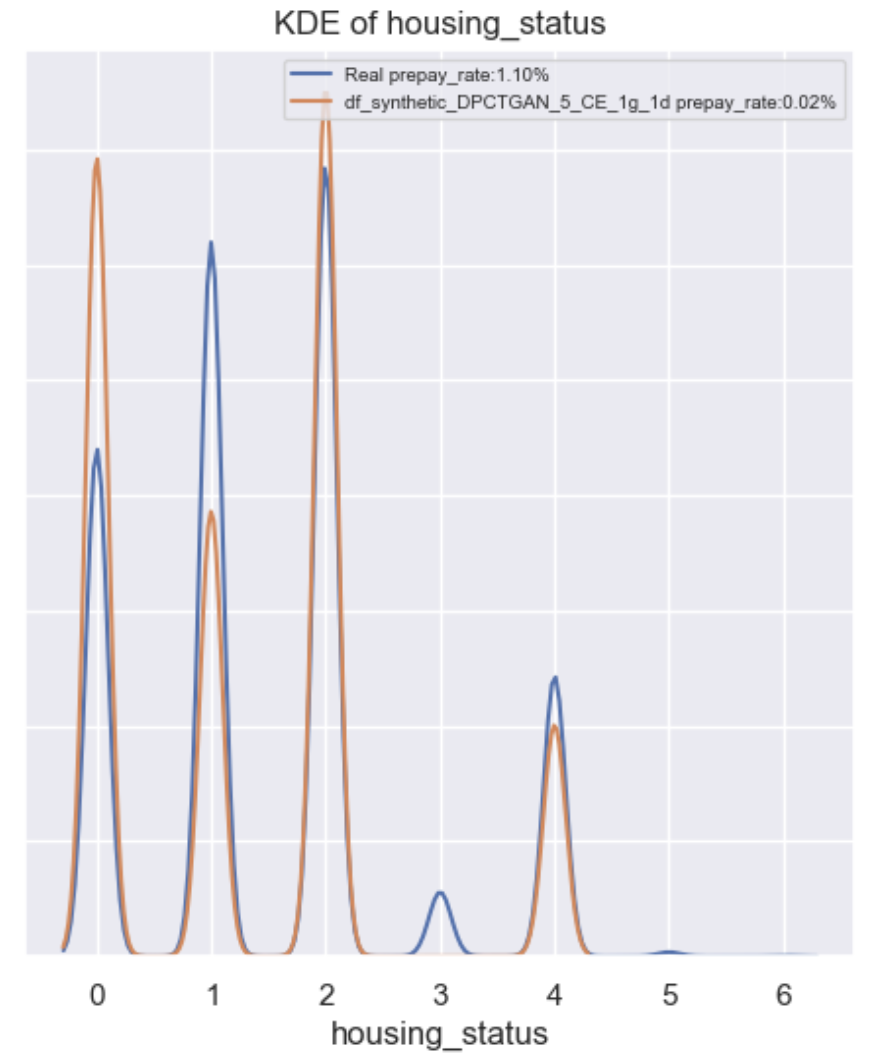
\includegraphics[width=0.5\linewidth]{Housing_Status_KDE_Plot.png}
        \end{center}
        %TODO: add caption
           \caption{Real vs. Synthetic data KDE Plot: Housing Status}
        \label{fig:long}
        \label{fig:onecol}
    \end{figure}

    \item \textbf{Discussion on results}:
    \begin{itemize}
        \item In terms of ML Utility, the baseline model with EPS 5.0 is the champion model.
        \item Observing the KDE Plots, we notice that generated synthetic categorical features (e.g. Payment Type, Housing Status KDE Plots) show a close similarity to real data, whereas some continuous features exhibit mode collapse (e.g. Income KDE Plot shown above)
        \item Mode collapse can be rationalized by the fact that the real dataset is unbalanced. The mode collapse causes the synthesization of the label \verb'Fraud_Bool' to be 0.02\% compared to the real dataset of 1.10\%.
        \item We measured distributional similarity using PMSE Ratio. As expected, the champion model has the lowest PMSE Ratio.
    \end{itemize}


    \item \textbf{discussion on success / failure}:
    \begin{itemize}
        \item We were able to generate synthetic data which has similar ML utility as real dataset. Synthetic dataset AUC/ROC degreaded by 4.15\%, which is reasonable.
        \item However, we could not achieve a reasonable distributional similarity for continuous features (as evident by KDE plots)
        \item PMSE Ratio figures can also be improved with additional data and experimental setups.
        \item Training GANs is an exceptionally resource and time intensive exercise. Each expeiment took on average 12 hours to run. There is a scope to improve model performance with better resource and training/experimentation time.
    \end{itemize}

\end{itemize}

\begin{table*}
\begin{center}
\begin{tabular}{|l|c|p{8cm}|}
\hline
Student Name & Contributed Aspects & Details \\
\hline\hline
Krishna Kumar & Data Sourcing and selection of target data & Identify and Source Dataset from Kaggle. \\
Sumit Machwe & Exploratory Data Analysis (EDA) & Generate Correlation plots, identify categorical and continuous variables and reduce dimentionality for experimentation. \\
Sumit Machwe & DiffPriv Runtime Environment Setup & Setup the complex runtime with various dependent libraries and their specific versions. \\
Krishna Kumar & Baseline Model: Implementation & Implement DPCTGAN, PATECTGAN and QUAIL with default parameters and chosen epsilon using smartnoise library. \\
Sumit Machwe & ML Utility implementation & Implement calculations for Precion, Recall, F1-Score and AUC/ROC and compiling the results in dataframe. \\
Krishna Kumar & KDE Plot and PMSE Ratio implementation & Implement KDE Plot and PMSE Ratio to calculate distributional similarity. \\
Krishna/Sumit & Hyper parameter Tuning Experimentation Setup & Design experimentation framework for hyper-parameter tuning. \\
Sumit Machwe & Hyperparameter Tuning: Batch-1 & Run 6 experiments on DPCTGAN based on defined experimental setup. \\
Krishna Kumar & Hyperparameter Tuning: Batch-2 & Run 6 experiments on DPCTGAN based on defined experimental setup. \\
Krishna/Sumit & Results, Analysis and Report & Assimilate all experiment results, plots etc and develop the final report.\\

\hline
\end{tabular}
\end{center}
\caption{Contributions of team members.}
\label{tab:contributions}
\end{table*}


\section{Other Sections}

    \begin{figure}[ht]
    \begin{center}
       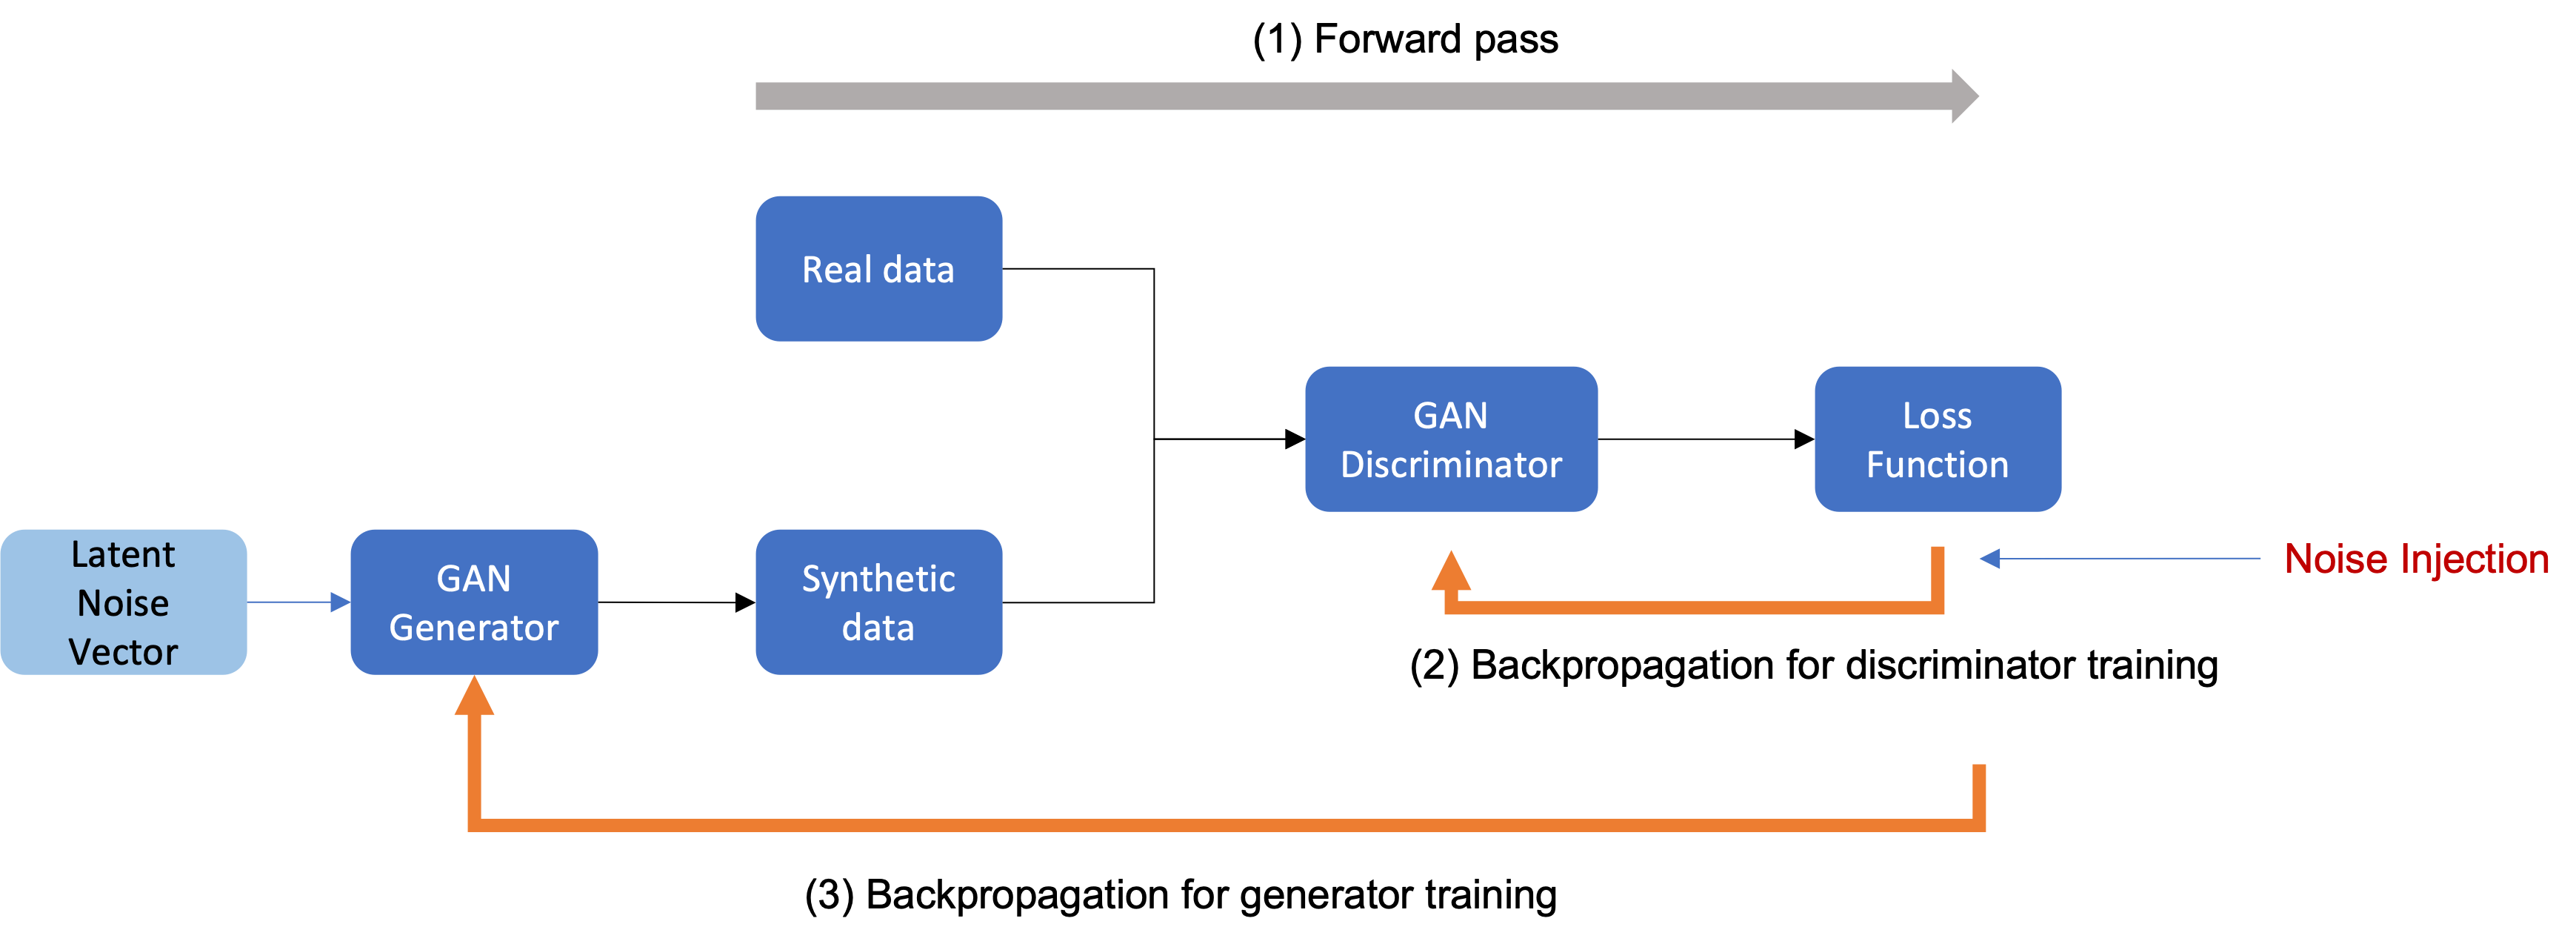
\includegraphics[width=0.9\linewidth]{DP-GAN-Framework.png}
    \end{center}
    %TODO: add caption
       \caption{GAN based models Architecture}.
    \label{fig:long}
    \label{fig:onecol}
    \end{figure}

\begin{itemize}
    \item Data Sourcing, EDA, Pre \& Post-Processing implementation of ML Utility and distributional plots (KDE Plots) are not based on deep-learning. However training the model using GANs (Generative Advarsarial Neural Networks) are based on deep learning and involves following hyper-parameter tuning:
    \begin{itemize}
        \item embedding layers
        \item learning rates
        \item epochs
        \item Generator depth
        \item Discriminator depths
        \item Sigma and Epsilon
    \end{itemize}

    %TODO: Remove this from Approach and put into Section# 4: Other Sections

    \item
    We used the open-source \href{https://github.com/opendp/smartnoise-sdk}{opendp/smartnoise-sdk} and the following Neural Network Synthesizers to train on the real data:

    \begin{itemize}
        \item \verb'DP-CTGAN': GAN-based synthesizer that uses conditional masks to learn tabular data.

        \item \verb'PATE-CTGAN': Conditional tabular GAN using Private Aggregation of Teacher Ensembles.

        \item \verb'QUAIL': Quailified Architecture to Improve Labeling. Divide epsilon in a known classification task between a differentially private synthesizer and classifier. Train DP classifier on real, fit DP synthesizer to features (excluding the target label), and use synthetic data from the DP synthesizer with the DP classifier to create artificial labels.

    \end{itemize}

    \item Pre-processing involved reducing the features and dataspace (11 features, 1 label and 300,000 records). This was input to the GAN network as an embedding.
    \item Output from learned GAN network was the synthetic data with same feature and record count as input data.
    \item \textbf{Loss Functions:}
    \begin{itemize}
        \item \verb'Cross-Entropy': is a metric used to measure how well a classification model in machine learning performs.
        \item \verb'Wasserstein': is a distance metric used in GANs to measure the difference between the generated and real data distributions, allowing for more stable training and improved quality of generated samples.
    \end{itemize}

    \item
    For \verb'TSTS' our model overfit. And hence, we decided to use \verb'TSTR' as our baseline metrics for ML Utility comparison. Please refer to Approach section for further details.

    \item Future potential: Tuning GANs is resource intensive. Any GAN based approach that optimizes or improves the training time will improve differential privacy framework and its applicability to the real world.
    \item Currently Differential Privacy algorithms are not generalizable across datasets. Further research is required to develop generic algorithm(s) for data synthesization using differential privacy.

    \item Project Repository: https://github.gatech.edu/cs7643-spring-2023/differential-privacy
\end{itemize}

\section{Work Division}
 \ref{tab:contributions}.

\newpage
\newpage

%-------------------------------------------------------------------------
% {\small
% \bibliographystyle{ieee_fullname}
% \bibliography{egbib}
% }

\begin{thebibliography}{9}
  \bibitem{1}\text{Kaggle Dataset: }\href{https://www.kaggle.com/datasets/sgpjesus/bank-account-fraud-dataset-neurips-2022}{https://www.kaggle.com/datasets/sgpjesus/bank-account-fraud-dataset-neurips-2022}

  \bibitem{2} \text{Create privacy-preserving synthetic data for machine learning with SmartNoise }
  \href{https://cloudblogs.microsoft.com/opensource/2021/02/18/create-privacy-preserving-synthetic-data-for-machine-learning-with-smartnoise/}{https://cloudblogs.microsoft.com/opensource/2021/02/18/create-privacy-preserving-synthetic-data-for-machine-learning-with-smartnoise/}

  \bibitem{3}\text{10 Breakthrough Technologies 2020 }
  \href{https://www.technologyreview.com/10-breakthrough-technologies/2020/#differential-privacy}{https://www.technologyreview.com/10-breakthrough-technologies/2020/#differential-privacy}

  \bibitem{4} \text{Understanding Differential Privacy }
  \href{https://medium.com/towards-data-science/understanding-differential-privacy-85ce191e198a}{https://medium.com/towards-data-science/understanding-differential-privacy-85ce191e198a}

  \bibitem{5}\text{General and specific utility measures for synthetic data }
  \href{https://arxiv.org/pdf/1604.06651}{https://arxiv.org/pdf/1604.06651}

  \bibitem{6} \text{Quail Paper }
  \href{https://arxiv.org/abs/2011.05537}{https://arxiv.org/abs/2011.05537}

  \bibitem{7} \text{DP-GAN Paper }
  \href{https://arxiv.org/pdf/1808.00087.pdf}{https://arxiv.org/pdf/1808.00087.pdf}

   \bibitem{8}\text{PATE-GAN Paper }
  \href{https://openreview.net/forum?id=S1zk9iRqF7}{https://openreview.net/forum?id=S1zk9iRqF7}

  \bibitem{9}\text{CT-GAN Paper }
  \href{https://link.springer.com/chapter/10.1007/978-3-031-09342-5\_17}{https://link.springer.com/chapter/10.1007/978-3-031-09342-5\_17}

\end{thebibliography}
\end{document}
